%%%%%%%%%%%%%%%%%%%%%%%%%%%%%%%%%%%%%%%%%
% Daily Laboratory Book
% LaTeX Template
%
% This template has been downloaded from:
% http://www.latextemplates.com
%
% Original author:
% Frank Kuster (http://www.ctan.org/tex-archive/macros/latex/contrib/labbook/)
%
% Important note:
% This template requires the labbook.cls file to be in the same directory as the
% .tex file. The labbook.cls file provides the necessary structure to create the
% lab book.
%
% The \lipsum[#] commands throughout this template generate dummy text
% to fill the template out. These commands should all be removed when 
% writing lab book content.
%
% HOW TO USE THIS TEMPLATE 
% Each day in the lab consists of three main things:
%
% 1. LABDAY: The first thing to put is the \labday{} command with a date in 
% curly brackets, this will make a new page and put the date in big letters 
% at the top.
%
% 2. EXPERIMENT: Next you need to specify what experiment(s) you are 
% working on with an \experiment{} command with the experiment shorthand 
% in the curly brackets. The experiment shorthand is defined in the 
% 'DEFINITION OF EXPERIMENTS' section below, this means you can 
% say \experiment{pcr} and the actual text written to the PDF will be what 
% you set the 'pcr' experiment to be. If the experiment is a one off, you can 
% just write it in the bracket without creating a shorthand. Note: if you don't 
% want to have an experiment, just leave this out and it won't be printed.
%
% 3. CONTENT: Following the experiment is the content, i.e. what progress 
% you made on the experiment that day.
%
%%%%%%%%%%%%%%%%%%%%%%%%%%%%%%%%%%%%%%%%%

%----------------------------------------------------------------------------------------
%	PACKAGES AND OTHER DOCUMENT CONFIGURATIONS
%----------------------------------------------------------------------------------------

\documentclass[idxtotoc,hyperref,openany]{labbook} % 'openany' here removes the gap page between days, erase it to restore this gap; 'oneside' can also be added to remove the shift that odd pages have to the right for easier reading

\usepackage[ 
  backref=page,
  pdfpagelabels=true,
  plainpages=false,
  colorlinks=true,
  bookmarks=true,
  pdfview=FitB]{hyperref} % Required for the hyperlinks within the PDF
  
\usepackage{booktabs} % Required for the top and bottom rules in the table
\usepackage{float} % Required for specifying the exact location of a figure or table
\usepackage{graphicx} % Required for including images
\usepackage{lipsum} % Used for inserting dummy 'Lorem ipsum' text into the template

\newcommand{\HRule}{\rule{\linewidth}{0.5mm}} % Command to make the lines in the title page
\setlength\parindent{0pt} % Removes all indentation from paragraphs

\graphicspath{{../reports/figures/}} % Sets the path for all graphics, so only name is needed afterwards.

%----------------------------------------------------------------------------------------
%	DEFINITION OF EXPERIMENTS
%----------------------------------------------------------------------------------------

%\newexperiment{example}{This is an example experiment}
%\newexperiment{example2}{This is another example experiment}
\newexperiment{First steps}{}
\newexperiment{Data cleaning}{}
\newexperiment{table}{This shows a sample table}
%\newexperiment{shorthand}{Description of the experiment}

%---------------------------------------------------------------------------------------

\begin{document}

%----------------------------------------------------------------------------------------
%	TITLE PAGE
%----------------------------------------------------------------------------------------

\frontmatter % Use Roman numerals for page numbers
\title{
\begin{center}
\HRule \\[0.4cm]
{\Huge \bfseries Lab Book \\[0.5cm] \Large Machine Learning}\\[0.4cm] % Degree
\HRule \\[1.5cm]
\end{center}
}
\author{\Huge C\'ordoba Romero, Javier \\ \Huge Corroto Mart\'in, Juan Jos\'e \\ \Huge Guerrero del Pozo, \'Alvaro \\ \\[2cm]} % Your name and email address
\date{Beginning 10 October 2018} % Beginning date
\maketitle

\tableofcontents

\mainmatter % Use Arabic numerals for page numbers

%----------------------------------------------------------------------------------------
%	LAB BOOK CONTENTS
%----------------------------------------------------------------------------------------

% Blank template to use for new days:

%\labday{Day, Date Month Year}

%\experiment{}

%Text

%-----------------------------------------

%\experiment{}

%Text

%----------------------------------------------------------------------------------------

\labday{Wednesday, 10 October 2018}
\experiment{First steps}

Done by Juan Jos\'e Corroto, Javier C\'ordoba and \'Alvaro Guerrero\\

We've initialized the repo with \texttt{coookiecutter} directory structure and learnt the purpose of each directory.
We've also learnt how to work with \texttt{pandas}, read and write a csv and how to work with spyder.

%----------------------------------------------------------------------------------------

\experiment{Data cleaning}

We've picked the data of only the first day, we've done this by looking at the raw data and looking at the column \textit{"TimeStemp"}.

Then we've deleted the \textit{UUID, Version} and \textit{TimeStemp} columns because they were non-numerical values.

Then we've tried deleting the rows that had \textit{NaN} values, and we ended up deleting the whole dataframe. So, after scanning the dataframe, we have realized that the columns 
\begin{enumerate}
\item \textit{RotationVector\_cosThetaOver2\_MEAN}
\item \textit{RotationVector\_cosThetaOver2\_MEDIAN}
\item \textit{RotationVector\_cosThetaOver2\_MIDDLE\_SAMPLE}
\end{enumerate}
Had all their values as \textit{Nan}.
\\
After eliminating these 3 columns, we proceeded as before: we eliminated those rows that had \textit{NaN} values and deleted 2 rows.

Then we saved this new data as processed data in its corresponding folder: data/interim/.

%----------------------------------------------------------------------------------------


\labday{Wednesday, 17 October 2018}
\experiment{More cleaning}

Done by Juan Jos\'e Corroto, Javier C\'ordoba and \'Alvaro Guerrero\\

First, we have modified how we pick the first day data: instead of getting the 2038 first rows, we convert the \textit{'Timestemp'} to days and choosing the day 28 (the first one).\\

In addition to the columns dropped the last week, we have also dropped \textit{UUID}. Then every \textit{FFT} and \textit{Middle Sample} rows have been dropped too.\\

We have chosen just two sensors to do an initial exploration: \textbf{Accelerometer} and \textbf{Linear acceleration}. The purpose is to try and explore the data related to the movement of the phone.\\
So, we create a new dataframe with only \textit{Acelerometer} and \textit{Linear Aceleration}. Finally, we drop \textit{Covariances}, as we don't think they will be useful cause they are calculated as the relation \textit{2-by-2} of the axis.

\experiment{Visualization - Clustering}

We then calculate the \textit{PCA} with an \textit{explained\_variance\_ratio} of \textbf{0.78} and \textbf{0.14}, which is a very good representation of the original 18 features we were studying.

With this results, we plot a \textit{scatterplot} to visualize it.


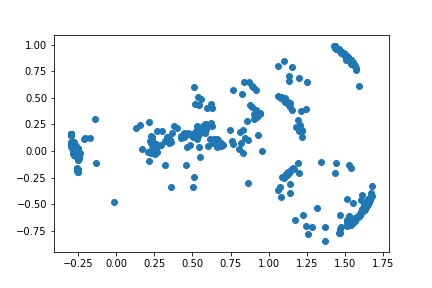
\includegraphics[scale=0.9]{PCA_Plot_Accelerometer_Day1.png}


After that we run the \textit{k-means} with different number of centroids and print the \textit{silhouette} and \textit{distortion}. Next we have the measurements of distortion and silhouette of KMeans with different number of centroids.

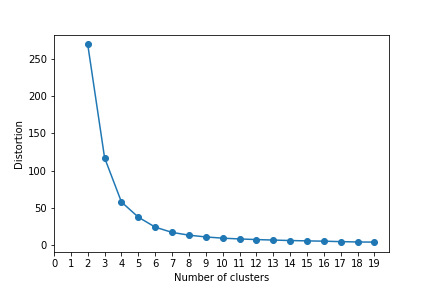
\includegraphics[scale=1]{KMeans_Distortion_Accelerometer_Day1.png}
\\

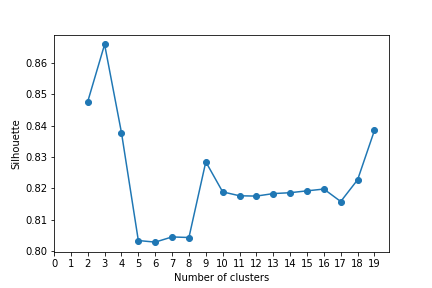
\includegraphics[scale=0.9]{KMeans_Silhouette_Accelerometer_Day1.png}
\\


By looking at the plots, we have decided to choose \textbf{4} as the final number of centroids.\\↔

\newpage
Finally, we run the \textit{k-means} algorithm with said number of centroids and plot the results, each cluster having a different color, and the centroids being colored in red.\\

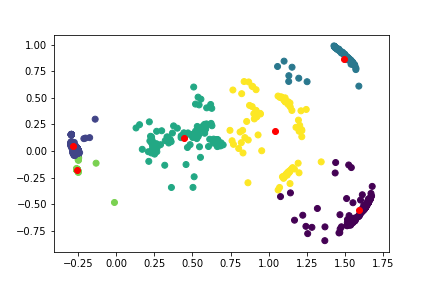
\includegraphics[scale=1]{KMeans_Plot_Accelerometer_Day1.png}
\\

%----------------------------------------------------------------------------------------

\labday{Friday, 26 March 2010}

\experiment{table}

\begin{table}[H]
\begin{tabular}{l l l}
\toprule
\textbf{Groups} & \textbf{Treatment X} & \textbf{Treatment Y} \\
\toprule
1 & 0.2 & 0.8\\
2 & 0.17 & 0.7\\
3 & 0.24 & 0.75\\
4 & 0.68 & 0.3\\
\bottomrule
\end{tabular}
\caption{The effects of treatments X and Y on the four groups studied.}
\label{tab:treatments_xy}
\end{table}

Table \ref{tab:treatments_xy} shows that groups 1-3 reacted similarly to the two treatments but group 4 showed a reversed reaction.

%----------------------------------------------------------------------------------------

\labday{Saturday, 27 March 2010}

\experiment{Bulleted list example} % You don't need to make a \newexperiment if you only plan on referencing it once

This is a bulleted list:

\begin{itemize}
\item Item 1
\item Item 2
\item \ldots and so on
\end{itemize}

%-----------------------------------------

\experiment{example}

\lipsum[6]

%-----------------------------------------

\experiment{example2}

\lipsum[7]

%----------------------------------------------------------------------------------------
%	FORMULAE AND MEDIA RECIPES
%----------------------------------------------------------------------------------------

\labday{} % We don't want a date here so we make the labday blank

\begin{center}
\HRule \\[0.4cm]
{\huge \textbf{Formulae and Media Recipes}}\\[0.4cm] % Heading
\HRule \\[1.5cm]
\end{center}

%----------------------------------------------------------------------------------------
%	MEDIA RECIPES
%----------------------------------------------------------------------------------------

\newpage

\huge \textbf{Media} \\ \\

\normalsize \textbf{Media 1}\\
\begin{table}[H]
\begin{tabular}{l l l}
\toprule
\textbf{Compound} & \textbf{1L} & \textbf{0.5L}\\
\toprule
Compound 1 & 10g & 5g\\
Compound 2 & 20g & 10g\\
\bottomrule
\end{tabular}
\caption{Ingredients in Media 1.}
\label{tab:med1}
\end{table}

%-----------------------------------------

%\textbf{Media 2}\\ \\

%Description

%----------------------------------------------------------------------------------------
%	FORMULAE
%----------------------------------------------------------------------------------------

\newpage

\huge \textbf{Formulae} \\ \\

\normalsize \textbf{Formula 1 - Pythagorean theorem}\\ \\
$a^2 + b^2 = c^2$\\ \\

%-----------------------------------------

%\textbf{Formula X - Description}\\ \\

%Formula

%----------------------------------------------------------------------------------------

\end{document}